\chapter{Siła opresji}
\AddToShipoutPictureBG*{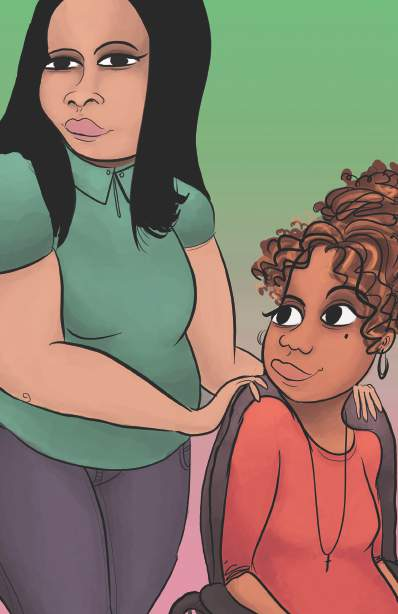
\includegraphics[width=\paperwidth,height=\paperheight]{TeX_files/2-0.png}}
\begin{flushright}
\vfill\textcolor{white}{Artist: Mohammed Fayaz}
\end{flushright}

\newpage
\begin{figure}[h]
\centering
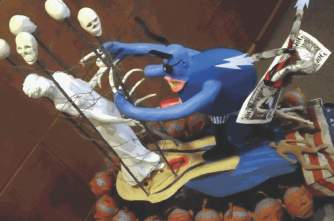
\includegraphics[width=16cm]{TeX_files/2-1.png}
\label{2-1}
\begin{flushright}
Artysta: JW Arndt
\end{flushright}
\end{figure}


\noindent\textcolor{ProcessBlue}{\textbf{\Large{W jaki sposób opresja wpływa na twoje uczucia?}}}\\
\large{\textbf{Oto emocje, które zidentyfikowaliśmy:}}
\begin{multicols}{3}
\begin{itemize}
\item[$\square$]{Rozzłoszczony}
\item[$\square$]{Niespokojny}
\item[$\square$]{Emocjonalnie wyczerpany}
\item[$\square$]{Rozwścieczony}
\item[$\square$]{Smutny}
\item[$\square$]{Zrozpaczony}
\item[$\square$]{Zasmucony}
\item[$\square$]{Bezradny}
\item[$\square$]{Bezsilny}
\item[$\square$]{Zawstydzony}
\item[$\square$]{Zmartwiony}
\item[$\square$]{Zakłopotany}
\item[$\square$]{Sfrustrowany}
\item[$\square$]{Bezwartościowy}
\item[$\square$]{Zaniepokojony}
\item[$\square$]{Zdradzony}
\item[$\square$]{Zmieszany}
\item[$\square$]{Izolujący się}
\item[$\square$]{Fizycznie wyczerpany}
\item[$\square$]{Buntowniczy}
\item[$\square$]{Odczuwający pustkę}
\item[$\square$]{Upokorzony}
\item[$\square$]{Nieufny}
\item[$\square$]{Zdenerwowany}
\item[$\square$]{Przygnębiony}
\item[$\square$]{Zdezorientowany}
\item[$\square$]{Defensywny}
\item[$\square$]{Oburzony}
\item[$\square$]{Niecierpliwy}
\item[$\square$]{Wrogi}
\item[$\square$]{Spięty}
\item[$\square$]{Zraniony}
\item[$\square$]{Rozczarowany}
\item[$\square$]{Wyobcowany}
\end{itemize}
\end{multicols}


\newpage
\noindent
\textcolor{ProcessBlue}{\textbf{\Large{Jakie inne emocje odczuwasz, kiedy doświadczasz opresji?}}}\\\\
\noindent\rule{\textwidth}{1pt}\\
\noindent\rule{\textwidth}{1pt}\\
\noindent\rule{\textwidth}{1pt}\\
\noindent\rule{\textwidth}{1pt}\\
\noindent\rule{\textwidth}{1pt}\\
\noindent\rule{\textwidth}{1pt}\\
\noindent\rule{\textwidth}{1pt}\\
\noindent\rule{\textwidth}{1pt}\\\\

\noindent\textcolor{ProcessBlue}{\textbf{\Large{W jaki sposób opresja wpływa na twoje zachowanie?}}}\\
\textbf{\large{Oto sposoby, które opisaliśmy:}}
\begin{multicols}{2}
\begin{itemize}
\item[$\square$]{Ukrywam się.}
\item[$\square$]{Przejadam się.}
\item[$\square$]{Nie jestem w stanie jeść.}
\item[$\square$]{Uciekam w sen.}
\item[$\square$]{Cierpię na bezsenność.}
\item[$\square$]{Atakuję.}
\item[$\square$]{Potrzebuję fizycznego dystansu od ludzi.}
\item[$\square$]{Zachowuję się jak szalony.}
\item[$\square$]{Staję się uległy.}
\item[$\square$]{Staję się brutalny.}
\item[$\square$]{Zastygam w bezruchu.}
\item[$\square$]{Przestaję rozmawiać.}
\item[$\square$]{Jąkam się.}
\item[$\square$]{Załamuję się emocjonalnie.}
\item[$\square$]{Przestaję o siebie dbać.}
\item[$\square$]{Mam koszmary.}
\item[$\square$]{Jestem biernie agresywny.}
\item[$\square$]{Chcę się odegrać.}
\item[$\square$]{Boję się przyszłości.}
\item[$\square$]{Czuję, że moje życie się rozpada.}
\item[$\square$]{Izoluję się.}
\item[$\square$]{Stosuję uniki.}
\item[$\square$]{Wycofuję się.}
\item[$\square$]{Uciekam w świat wyobraźni.}
\item[$\square$]{Trzęsę się.}
\item[$\square$]{Zastygam w bezruchu.}
\end{itemize}
\end{multicols}


\newpage
\noindent
\textcolor{ProcessBlue}{\textbf{\Large{W jaki sposób opresja wpływa na to, jak się zachowujesz?}}}\\\\
\noindent\rule{\textwidth}{1pt}\\
\noindent\rule{\textwidth}{1pt}\\
\noindent\rule{\textwidth}{1pt}\\
\noindent\rule{\textwidth}{1pt}\\
\noindent\rule{\textwidth}{1pt}\\
\noindent\rule{\textwidth}{1pt}\\
\noindent\rule{\textwidth}{1pt}\\
\noindent\rule{\textwidth}{1pt}\\\\

\noindent\textcolor{ProcessBlue}{\textbf{\Large{W jaki sposób opresja sprawia, że jest ci źle?}}}\\
\textbf{\large{Oto sposoby, które zidentyfikowaliśmy:}}
\begin{multicols}{2}
\begin{itemize}
\item[$\square$]{Próbowałam/Próbowałem popełnić samobójstwo.}
\item[$\square$]{Mam myśli samobójcze.}
\item[$\square$]{Mam ataki paniki.}
\item[$\square$]{Mam bóle głowy.}
\item[$\square$]{Mam bóle brzucha.}
\item[$\square$]{Doświadczam depresji.}
\item[$\square$]{Odczuwam niepokój i paranoję.}
\item[$\square$]{Mam nieustanne negatywne myśli.}
\item[$\square$]{Odczuwam zawroty głowy.}
\item[$\square$]{Mam zaburzenia odżywiania.}
\item[$\square$]{Nadużywam alkoholu i/lub narkotyków.}
\item[$\square$]{Mam koszmary.}
\item[$\square$]{Doświadczam zakłócenia snu.}
\item[$\square$]{Mam wrzody.}
\item[$\square$]{Nasilają się wszelkie moje symptomy.}
\item[$\square$]{Lęk i paranoiczna ochrona zdrowia.}
\item[$\square$]{Dokonuję samookaleczeń.}
\item[$\square$]{Nienawiść do siebie.}
\item[$\square$]{Cierpię na bezsenność.}
\item[$\square$]{Dochodzi do epizodów maniakalnych.}
\item[$\square$]{Doświadczam PTSD (posttraumatic stress disorder -- zespół stresu pourazowego).}
\item[$\square$]{Mam ,,urojenia''.}
\item[$\square$]{Mam ,,psychozy''.}
\item[$\square$]{Izoluję się.}
\item[$\square$]{Mam wysypkę.}
\item[$\square$]{Mam kompulsywne zachowania.}
\item[$\square$]{Wykazuję obsesyjne zachowania.}
\item[$\square$]{Mam depresję.}
\end{itemize}
\end{multicols}


\newpage
\noindent
\textcolor{ProcessBlue}{\textbf{\Large{W jaki sposób opresja manifestuje się w twoim ciele i~umyśle?}}}\\\\
\noindent\rule{\textwidth}{1pt}\\
\noindent\rule{\textwidth}{1pt}\\
\noindent\rule{\textwidth}{1pt}\\
\noindent\rule{\textwidth}{1pt}\\
\noindent\rule{\textwidth}{1pt}\\
\noindent\rule{\textwidth}{1pt}\\
\noindent\rule{\textwidth}{1pt}\\
\noindent\rule{\textwidth}{1pt}\\\\

\noindent\textcolor{ProcessBlue}{\textbf{\Large{W jaki sposób mikroagresja zagraża twojemu dobremu samopoczuciu?}}}\\
\textbf{\large{Oto, jak niektórzy z nas opisali to doświadczenie:}}
\begin{multicols}{2}
\begin{itemize}
\item[$\square$]{Wstyd za siebie.}
\item[$\square$]{Przyśpieszony puls.}
\item[$\square$]{Staję się naprawdę zdenerwowany lub wzburzony.}
\item[$\square$]{Wykazuję nadmierną agresję.}
\item[$\square$]{Staję się brutalny.}
\item[$\square$]{Dokonuję samookaleczeń.}
\item[$\square$]{Jestem przestraszony.}
\item[$\square$]{Jestem sfrustrowany.}
\item[$\square$]{Jest mi smutno i powraca fala wspomnień.}
\item[$\square$]{Rozpraszam się i tracę skupienie.}
\item[$\square$]{Nie radzę sobie.}
\item[$\square$]{Odczuwam niepokój.}
\item[$\square$]{Natrętne myśli.}
\item[$\square$]{Dzwonienie w uszach.}
\item[$\square$]{Uderzenia gorąca.}
\item[$\square$]{Flashbacki.}
\item[$\square$]{Wzburzenie.}
\item[$\square$]{Lęk.}
\item[$\square$]{Smutek.}
\item[$\square$]{Niepokój.}
\item[$\square$]{Nadmierna czujność.}
\item[$\square$]{Przyśpieszenie pulsu.}
\item[$\square$]{Złość.}
\item[$\square$]{Dezorientacja.}
\item[$\square$]{Zawroty głowy.}
\item[$\square$]{Mdłości.}
\item[$\square$]{Drżenie.}
\end{itemize}
\end{multicols}


\newpage
\noindent
\textcolor{ProcessBlue}{\textbf{\Large{W jakie inne sposoby mikroagresja zagraża twojemu dobremu samopoczuciu?}}}\\
\noindent\rule{\textwidth}{1pt}\\
\noindent\rule{\textwidth}{1pt}\\
\noindent\rule{\textwidth}{1pt}\\
\noindent\rule{\textwidth}{1pt}\\
\noindent\rule{\textwidth}{1pt}\\
\noindent\rule{\textwidth}{1pt}\\
\noindent\rule{\textwidth}{1pt}\\
\noindent\rule{\textwidth}{1pt}\\
\noindent\rule{\textwidth}{1pt}\\\\

\noindent\textcolor{ProcessBlue}{\textbf{\Large{W jaki sposób opresja wpływa na to, jak widzisz siebie?}}}\\
\textbf{\large{Oto sposoby, które zidentyfikowaliśmy:}}
\begin{multicols}{2}
\begin{itemize}
\item[$\square$]{Jest mi ze sobą źle.}
\item[$\square$]{Czuję, że lepiej, aby mnie tu nie było.}
\item[$\square$]{Staję się egocentryczna/egocentryczny.}
\item[$\square$]{Złoszczę się na siebie.}
\item[$\square$]{Nienawidzę siebie.}
\item[$\square$]{Wpadam w próbę dopasowania się do ideału samego/samej siebie, zamiast uczciwie być sobą.}
\item[$\square$]{Kwestionuję swoją zdolność do osiągania celów.}
\item[$\square$]{Kwestionuję to, że kiedykolwiek osiągnę szczęście.}
\item[$\square$]{Obawiam się, że nie jestem ,,wart''/ ,,warta'' bycia kochaną/kochanym.}
\item[$\square$]{Czuję się podkopywana/podkopywany.}
\item[$\square$]{Zastanawiam się, czy po prostu wszystko robię źle, co szybko prowadzi do gorszego samopoczucia.}
\item[$\square$]{Czuję się zdystansowany od siebie, rozbity i niepewny przyszłości.}
\item[$\square$]{Czuję się nieskupiony i wycofany.}
\item[$\square$]{Obwiniam siebie.}
\item[$\square$]{Mam myśli, że ,,trzeba było tego robić!”.}
\item[$\square$]{Ciężko jest mi czuć się silną/silnym i skuteczną/skutecznym w świecie.}
\item[$\square$]{Za każdym razem, gdy to się dzieje, muszę na nowo nawiązywać relację ze sobą.}
\item[$\square$]{Wstyd i nienawiść towarzyszą mi, bardzo ciężko jest je zostawić za sobą.}
\item[$\square$]{Wstyd i nienawiść towarzyszą mi, bardzo ciężko jest je zostawić za sobą.}
\item[$\square$]{Obserwuję, jak mój umysł wiruje od złości, winy i frustracji.}
\item[$\square$]{Wątpię w siebie.}
\item[$\square$]{Mam obniżoną pewność siebie w odniesieniu do moich możliwości wchodzenia w interakcje z innymi o oceniania innych.}
\item[$\square$]{Czuję się zdesperowany i bezwartościowy, analizując dawne krzywdy.}
\item[$\square$]{Nie umiem radzić sobie z myślami o przyszłych krzywdach.}
\item[$\square$]{Mam przełączenie i ,,zmiany'', które mogą wyglądać jak wahania nastroju, lecz nimi nie są.}
\item[$\square$]{Często zmagam się z nienawiścią do siebie i wstydem.}
\item[$\square$]{Czuję się ,,mniej niż'' i gorszy od swoich rówieśników.}
\item[$\square$]{Często czuję się wyobcowana/wyobcowany od siebie.}
\end{itemize}
\end{multicols}

\begin{figure}[h]
\centering
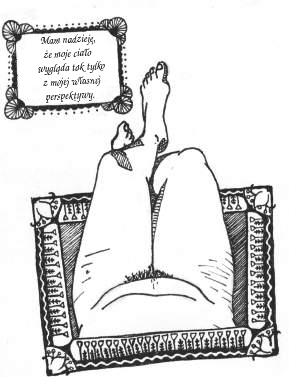
\includegraphics[height=16cm]{TeX_files/2-2-napis.png}
\label{2-2}
\begin{flushright}
Artysta: Jodi Bentivegna
\end{flushright}
\end{figure}

\newpage
\noindent
\textcolor{ProcessBlue}{\textbf{\Large{W jaki sposób opresja wpływa na to, jak postrzegasz siebie?}}}\\
\noindent\rule{\textwidth}{1pt}\\
\noindent\rule{\textwidth}{1pt}\\
\noindent\rule{\textwidth}{1pt}\\
\noindent\rule{\textwidth}{1pt}\\
\noindent\rule{\textwidth}{1pt}\\
\noindent\rule{\textwidth}{1pt}\\
\noindent\rule{\textwidth}{1pt}\\
\noindent\rule{\textwidth}{1pt}\\\\

\noindent\textcolor{ProcessBlue}{\textbf{\Large{Jakie są społeczne konsekwencje opresji?}}}\\
\textbf{\large{Wpływa ona na nasze relacje z przyjaciółmi, rodziną i partnerami w następujący sposób:}}
\begin{multicols}{2}
\begin{itemize}
\item[$\square$]{Nie mam przyjaciół.}
\item[$\square$]{Moja rodzina nie rozmawia ze mną.}
\item[$\square$]{Izoluję się.}
\item[$\square$]{W złości atakuję swoją rodzinę i przyjaciół.}
\item[$\square$]{Kiedy zacząłem/zaczęłam być otwarta/otwarty, moja rodzina zaczęła traktować mnie jak czarny charakter i mówić mi, że jestem samolubna/samolubny.}
\item[$\square$]{Przyjaciele, którzy nie rozumieją, czym jest opresja, nie znają mnie całkowicie, ponieważ nie widzą tego kontekstu.}
\item[$\square$]{Muszę zmagać się z moimi wewnętrznie uwarunkowanymi reakcjami na seks, które sygnalizują ,,uwaga, jesteś wykorzystywana/wykorzystywany'', tak abym mogła/mógł doświadczyć go w inny sposób (to znaczy pozytywny) lub nawet w ogóle go doświadczyć i nie być przejrzana/przejrzany.}
\item[$\square$]{Żywię urazę.}
\item[$\square$]{Sprawia, że jestem ostrożny.}
\item[$\square$]{Mam trudności w ufaniu sobie lub innym.}
\item[$\square$]{Sprawia, że komunikacja jest bardzo wymagająca.}
\item[$\square$]{Sprawia, że ciężko jest mi czuć się komfortowo w sytuacjach w grupie.}
\item[$\square$]{Mam trudności w utrzymywaniu kontaktów społecznych i odczuwaniu bezpieczeństwa przy wyrażaniu emocji wśród innych.}
\item[$\square$]{Czasami zachowuję się, jakbym był/była poddawana/poddawany opresji w relacjach, nawet, jeśli nie jestem.}
\end{itemize}
\end{multicols}


\newpage
\noindent
\textbf{\large{Wpływa ona na naszą szerszą społeczność w następujący sposób:}}
\begin{multicols}{2}
\begin{itemize}
\item[$\square$]{Izoluję się.}
\item[$\square$]{Jestem wyobcowany od wszystkich z wyjątkiem swoich rówieśników.}
\item[$\square$]{Nadal jest mi ciężko uwierzyć, że zostanę zaakceptowany i obdarzony zaufaniem przez ludzi.}
\item[$\square$]{Moje kręgi są raczej małe i nie nawiązuję relacji, od czasu gdy byłam/byłem młodsza/młodszy.}
\item[$\square$]{Czasami zdaję sobie sprawę, że zabiera mi dużo czasu osiągnięcie tego, co inni ludzie mogą postrzegać jako proste komunikaty.}
\item[$\square$]{Ograniczam to, jak często wchodzę w interakcje z ludźmi wokół mnie w miejscach publicznych i w społeczności z powodu mojego braku pewności siebie i lęku przed byciem nieakceptowanym lub nieszanowanym.}
\item[$\square$]{Poczucie, że nie mogę oczekiwać poczucia bezpieczeństwa w szerszym świecie, sprawia, że jestem bojaźliwa/bojaźliwy i pół-obecna/pół-obecny.}
\item[$\square$]{Nie widzę sensu należenia do mojego szerszej społeczności.}
\item[$\square$]{Moje interakcje są ograniczone i powierzchowne. Przybieram uśmiechniętą twarz i pozostaję w szeregu.}
\item[$\square$]{Nie mogę pozwolić na to, by ktokolwiek poznał moje zmagania.}
\item[$\square$]{Jestem zupełnie przekonana/przekonany, że szersza społeczność gardzi mną i nie chce mieć ze mną nic wspólnego.}
\item[$\square$]{Czuję, że nie mam nic do zaoferowania, dania lub zrobienia.}
\item[$\square$]{Sprawia, że ciężko jest znaleźć miejsce i sposób, by sensownie działać na rzecz społeczności.}
\end{itemize}
\end{multicols}

\noindent
\textcolor{ProcessBlue}{\textbf{\Large{Jakich innych społecznych konsekwencji opresji doświadczasz?}}}\\
\noindent\rule{\textwidth}{1pt}\\
\noindent\rule{\textwidth}{1pt}\\
\noindent\rule{\textwidth}{1pt}\\
\noindent\rule{\textwidth}{1pt}\\
\noindent\rule{\textwidth}{1pt}\\
\noindent\rule{\textwidth}{1pt}\\
\noindent\rule{\textwidth}{1pt}\\
\noindent\rule{\textwidth}{1pt}\\
\noindent\rule{\textwidth}{1pt}\\\\


\newpage
\begin{figure}[h]
\centering
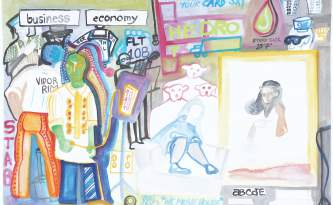
\includegraphics[width=14cm]{TeX_files/2-3.png}
\label{2-2}
\begin{flushright}
Artysta: Eddy Falconer
\end{flushright}
\end{figure}

\noindent\textcolor{ProcessBlue}{\textbf{\Large{W jaki sposób opresja wpływa na twoją zdolność do pracy?}}}\\
\textbf{\large{Oto sposoby, które zidentyfikowaliśmy:}}
\begin{multicols}{2}
\begin{itemize}
\item[$\square$]{Nie mogę pracować, kiedy śpię 24 godziny na dobę przez 7 dni w tygodniu.}
\item[$\square$]{Leki sprawiają, że jest mi trudniej sprawiać naturalne wrażenie podczas wchodzenia w interakcje ze współpracownicami/współpracownikami i kolegami/koleżankami z klasy.}
\item[$\square$]{Nieustannie porzucam swoje prace, ponieważ istnieją zachowania, które nasilają moje okresy depresji i nie mogę dobrze wykonywać swojej pracy.}
\item[$\square$]{Miałam/Miałem 42 prace. Jest niemal cholernie niemożliwe, bym trzymał/trzymała się jednej. Mimo wysokich kwalifikacji i odporności oraz mocnych kontaktów zawodowych, nie mogę utrzymać się w pracy na bardzo długo.}
\item[$\square$]{Szczerze mówiąc, nie wiem nawet, w jaki sposób naprawdę mogłabym/mógłbym pracować... Choć oczywiście nie mogę nie pracować, więc panuje ciągły, bolesny bałagan.}
\item[$\square$]{Próba wejścia w interakcje z ludźmi, którzy nie rozumieją i nie chcą rozumieć, sprawia, że mam ochotę się poddać, więc skupiam się dużo na sobie i robię co w mojej mocy, by znaleźć pracę, która nie wymaga do tego innych ludzi.}
\item[$\square$]{Nie mogę dłużej pracować. Podejrzewam, że jest to reakcja na opresję.}
\item[$\square$]{Często odczuwam osłabiający niepokój związany z PTSD i przez to trzymałam/trzymałem się prac w niepełnym wymiarze godzin, jako że obawiam się brania zbyt dużej odpowiedzialności.}
\item[$\square$]{Obawiam się ataków i tego, że nie będę w stanie wyjaśnić, dlaczego nie mogę pracować.}
\end{itemize}
\end{multicols}


\newpage
\noindent
\textcolor{ProcessBlue}{\textbf{\Large{W jaki sposób opresja wpływa na twoje codzienne życie i twoją zdolność do pracy?}}}\\
\noindent\rule{\textwidth}{1pt}\\
\noindent\rule{\textwidth}{1pt}\\
\noindent\rule{\textwidth}{1pt}\\
\noindent\rule{\textwidth}{1pt}\\
\noindent\rule{\textwidth}{1pt}\\
\noindent\rule{\textwidth}{1pt}\\
\noindent\rule{\textwidth}{1pt}\\
\noindent\rule{\textwidth}{1pt}\\
\noindent\rule{\textwidth}{1pt}\\\\

\noindent\textcolor{ProcessBlue}{\textbf{\Large{W jaki sposób opresja wpływa na twoje codzienne życie?}}}\\
\textbf{\large{Oto sposoby, które zidentyfikowaliśmy:}}
\begin{multicols}{2}
\begin{itemize}
\item[$\square$]{Czyni moje życie marginalnym, zdezorganizowanym i żałosnym.}
\item[$\square$]{Walka z przejadaniem się i innym autodestrukcyjnymi nawykami zabrała mi dużo czasu.}
\item[$\square$]{Choroba umysłowa jest niewidoczna.}
\item[$\square$]{Codzienne życie boli jak diabli.}
\item[$\square$]{Piętnaście lat leków przeciwpsychotycznych zebrało swoje żniwo.}
\item[$\square$]{Nieustanny ból.}
\item[$\square$]{Nieustanne opanowywanie mojego przelewającego się zbiornika.}
\item[$\square$]{Nieustanne zmartwienie i uczucie bycia ,,przegranym''.}
\item[$\square$]{Budzę się w depresji... Każdy dzień jest taki sam i nie ma nic do zrobienia i nikogo, z kim można by porozmawiać.}
\item[$\square$]{Zawsze szukam policji. Nie boję się ludzi z mojego sąsiedztwa, po prostu boję się policji, kiedy ją widzę.}
\item[$\square$]{Odkładam na później takie rzeczy jak sprzątanie czy mycie naczyń i zatracam się w internecie.}
\item[$\square$]{W moim codziennym życiu w każdej chwili jest dla mnie wyzwaniem, by doświadczyć mojej własnej perspektywy, poczuć się dobrze w swojej skórze, odkryć znaczenie, połączenie i sens, by dalej żyć.}
\item[$\square$]{Są dni, kiedy zwykłe wstanie z łóżka sprawia, że chce mi się płakać.}
\item[$\square$]{Konieczność opuszczenia domu niemal zawsze łamie mi serce.}
\item[$\square$]{Bycie odpowiedzialną/odpowiedzialnym jest trudne. Ciężko jest zadbać o siebie.}
\end{itemize}
\end{multicols}


\newpage
\noindent
\noindent\rule{\textwidth}{1pt}\\
\noindent\rule{\textwidth}{1pt}\\
\noindent\rule{\textwidth}{1pt}\\
\noindent\rule{\textwidth}{1pt}\\
\noindent\rule{\textwidth}{1pt}\\
\noindent\rule{\textwidth}{1pt}\\
\noindent\rule{\textwidth}{1pt}\\
\noindent\rule{\textwidth}{1pt}\\
\noindent\rule{\textwidth}{1pt}\\
\noindent\rule{\textwidth}{1pt}\\
\noindent\rule{\textwidth}{1pt}\\
\noindent\rule{\textwidth}{1pt}\\
\noindent\rule{\textwidth}{1pt}\\
\noindent\rule{\textwidth}{1pt}\\
\noindent\rule{\textwidth}{1pt}\\
\noindent\rule{\textwidth}{1pt}\\
\noindent\rule{\textwidth}{1pt}\\
\noindent\rule{\textwidth}{1pt}\\
\noindent\rule{\textwidth}{1pt}\\
\noindent\rule{\textwidth}{1pt}\\
\noindent\rule{\textwidth}{1pt}\\
\noindent\rule{\textwidth}{1pt}\\
\noindent\rule{\textwidth}{1pt}\\
\noindent\rule{\textwidth}{1pt}\\
\noindent\rule{\textwidth}{1pt}\\
\noindent\rule{\textwidth}{1pt}\\
\noindent\rule{\textwidth}{1pt}\\
\noindent\rule{\textwidth}{1pt}\\
